\chapter{Significato di approssimare}
\section{L'idea di approssimazione}
Immagina di avere due insiemi di oggetti: uno di questi, chiamiamolo $\llbracket P \rrbracket$,
ha una caratteristica speciale che chiameremo $Q$. Ora, il punto cruciale è che non possiamo dire
con certezza se un determinato oggetto appartiene a $Q$ o meno. È come se avessimo un mucchio di
oggetti e non riuscissimo a dire se uno specifico oggetto appartiene a un gruppo particolare o meno.

Quello che dobbiamo fare è trovare un modo per approssimare l'insieme $\llbracket P \rrbracket$
in modo da poter prendere decisioni più facili su $Q$. In altre parole, dobbiamo trovare un altro
insieme, $\llbracket P \rrbracket^\sharp$, che contiene la maggior parte degli oggetti di $\llbracket P \rrbracket$,
ma che sia più facile da analizzare. Questo insieme deve avere due caratteristiche importanti: tutti gli
oggetti di $\llbracket P \rrbracket$ devono essere anche in $\llbracket P \rrbracket^\sharp$, e l'insieme
$\llbracket P \rrbracket^\sharp$ deve essere tale che possiamo dire con certezza se un oggetto appartiene a $Q$ o meno.

Quando abbiamo questo insieme $\llbracket P \rrbracket^\sharp$, possiamo utilizzarlo per fare deduzioni
su $Q$. Se tutti gli oggetti in $\llbracket P \rrbracket^\sharp$ appartengono a $Q$, allora possiamo dire
con sicurezza che tutti gli oggetti in $\llbracket P \rrbracket$ devono appartenere a $Q$. Ma se non
tutti gli oggetti in $\llbracket P \rrbracket^\sharp$ appartengono a $Q$, non possiamo essere certi se gli
oggetti in $\llbracket P \rrbracket$ appartengono o meno a $Q$.

In sostanza, il nostro obiettivo è rendere più facile prendere decisioni su questi oggetti, anche se non
possiamo dire con certezza assoluta se un oggetto specifico appartiene a $Q$. Questo approccio ci consente
di ragionare in modo più chiaro su questi insiemi e di trarre conclusioni ragionevoli su di essi.

La correttezza ci consente di sfruttare la decidibilità dell'approssimazione:
\[
  \llbracket P \rrbracket \subseteq Q \implies \llbracket P \rrbracket^\sharp \subseteq Q  
\]
Altrimenti, non possiamo saperlo con certezza!
\subsection{Astrazione della semantica}
Vediamo come costruire l'insieme $\llbracket P \rrbracket^\sharp$ a partire da $\llbracket P \rrbracket$.
Specificheremo la semantica come una coppia: una funzione $f$ (\textit{con punto fisso}) e un
dominio di calcolo $D$ (\textit{ordinato}).

\begin{itemize}
  \item Astrazione del dominio di calcolo e delle relazioni tra oggetti concreti e astratti, ovvero 
  l'osservazione astratta dei dati e come questi si relazionano tra loro.
  \item Astrazione del calcolo, con particolare attenzione all'astrazione del punto fisso, come la 
  semantica manipola questi risultati astratti.
\end{itemize}
L'astrazione è il processo di sostituire qualcosa di concreto con una descrizione che considera alcune proprietà
(\textit{generalmente non tutte}), definita come modello astratto.
Può descrivere alcune proprietà in modo preciso, ma non tutte.

Un'astrazione $\wp(\Sigma)$ di oggetti in $\Sigma$ è $A \subseteq \wp(\Sigma)$ tale che:
\begin{itemize}
    \item Gli elementi presenti nell'insieme $A$ sono quelli descritti precisamente
    dall'astrazione, senza perdita di precisione.
    \item Gli elementi non presenti nell'insieme $A$ devono essere rappresentati da
    altri elementi dell'insieme, con una perdita di precisione.
\end{itemize}
\subsection{Oggetti}
Nell'analisi/verifica dei programmi dobbiamo considerare oggetti che rappresentano parti dello stato di calcolo:
\begin{itemize}
    \item Valori: Booleani, Interi,... $\mathcal{V}$
    \item Nomi di variabili $\mathbb{X}$
    \item Ambienti $\mathbb{X} \rightarrow \mathcal{V}$
    \item Stacks
    \item $\ldots$
\end{itemize}
\subsubsection{Proprietà}
Le proprietà sono insiemi di oggetti (che hanno quella proprietà). Esempi:
\begin{itemize}
    \item Numeri naturali dispari: $\{1, 3, 4, \dots, 2n + 1, \dots\}$
    \item Numeri interi pari: $\{2z \mid z \in \mathbb{Z}\}$
    \item Valori delle variabili intere: $\{x \mid x \in \mathbb{X} \land \texttt{minint} < x < \texttt{maxint}\}$
    \item Proprietà di invarianza: di un programma con stati: $\Gamma$
    \[
      I \in \wp(\Sigma)
    \]
    \item $\ldots$
\end{itemize}
\subsection{Proprietà}
L'insieme delle proprietà di $\wp(\Sigma)$ degli oggetti in $\Sigma$ è un reticolo distributivo completo, 
\[
  \langle \wp(\Sigma), \subseteq, \varnothing, \sigma, \Sigma, \cup, \cap, \neg  \rangle 
\]
Nell'analisi di un sistema complesso, è essenziale considerare l'astrazione come un processo chiave
per semplificare la comprensione. Quando si tratta di approssimare una proprietà concreta con
un'astrazione, si aprono due possibili approcci.
L'approccio di \textbf{approssimazione dal basso} implica che l'astrazione rappresenti un sottoinsieme
della proprietà concreta,
mentre l'approccio di \textbf{approssimazione dall'alto} ($P$) implica che l'astrazione rappresenti un
sovrainsieme della proprietà concreta. Questi approcci possono essere visti come duali,
sebbene l'analisi si concentri principalmente sull'approccio di approssimazione dall'alto,
poiché trovare approssimazioni utili dal basso può essere più impegnativo e complesso.

\begin{figure}[H]
  \centering
  \begin{tikzpicture}[scale=0.8]
    % Nodes
    \node (top) at (0,2) {$\Sigma$};
    \node (a) at (-2,0) {$\alpha$};
    \node (b) at (2,0) {$\beta$};
    \node (bottom) at (0,-2) {$\varnothing$};
    % Lines
    \draw (top) -- (a) -- (bottom);
    \draw (top) -- (b) -- (bottom);
    \draw (a) -- (b);
  \end{tikzpicture}
\end{figure}
\subsubsection{Least upper bound}
Il least upper bound (\verb|LUB|) di un insieme di elementi è il più piccolo
elemento del reticolo che è maggiore o uguale a ciascun elemento dell'insieme ($X \lor Y$).
Ovvero in $\wp(D)$ tale che $A \supseteq X$ e $A \supseteq Y$.
\begin{figure}[H]
  \centering
  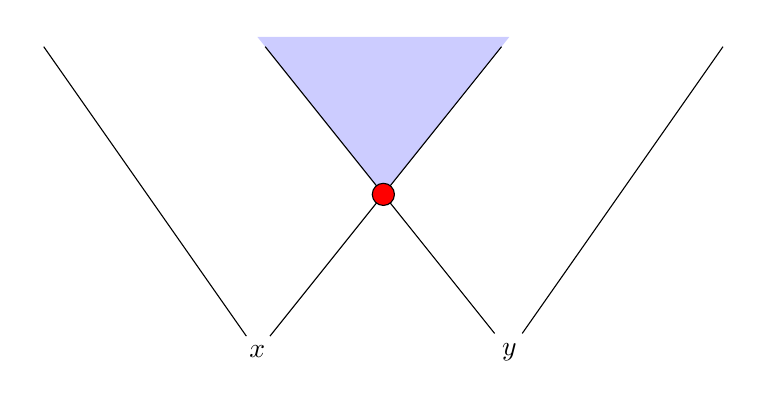
\begin{tikzpicture}[scale=0.8]
    % Nodes
    \node (from-y-to-x) at (-2, 5) {};
    \node (from-x-to-y) at (2, 5) {};
    \node (inters) at (0,2.5) {};
    \node (x-side) at (-5.5,5) {};
    \node (y-side) at (5.5,5) {};
    \node (x) at (-2,0) {$x$};
    \node (y) at (2,0) {$y$};

    %colorare l'area 
    \fill[blue!20] (0,2.5) -- (from-x-to-y.center) -- (from-y-to-x.center) -- cycle;
    

    % Lines
    \draw (x) -- (from-x-to-y);
    \draw (y) -- (from-y-to-x);
    \draw (x) -- (x-side);
    \draw (y) -- (y-side);

    \draw[fill=red] (0,2.5) circle (5pt);
    
  \end{tikzpicture}
\end{figure}
\subsubsection{Greatest lower bound}
Il greatest lower bound (\verb|GLB|) di un insieme di elementi è il più grande
elemento del reticolo che è minore o uguale a ciascun elemento dell'insieme ($X \land Y$).
Ovvero in $\wp(D)$ tale che $A \subseteq X$ e $A \subseteq Y$.
\begin{figure}[H]
  \centering
  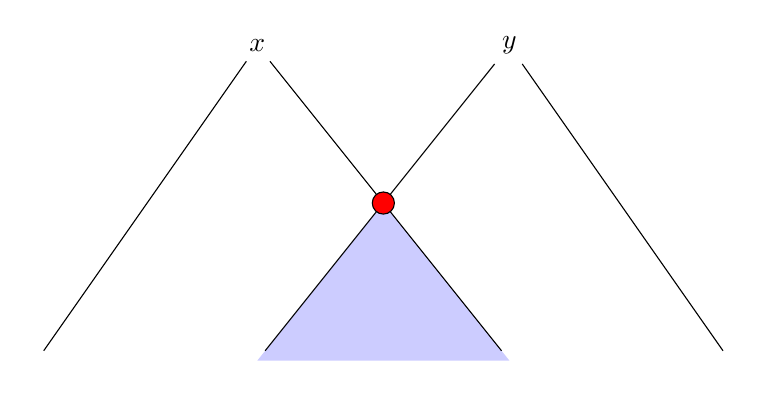
\begin{tikzpicture}[scale=0.8]
    % Nodes
    \node (from-y-to-x) at (-2, -5) {};
    \node (from-x-to-y) at (2, -5) {};
    \node (inters) at (0,-2.5) {};
    \node (x-side) at (-5.5,-5) {};
    \node (y-side) at (5.5,-5) {};
    \node (x) at (-2,0) {$x$};
    \node (y) at (2,0) {$y$};

    %colorare l'area 
    \fill[blue!20] (0,-2.5) -- (from-x-to-y.center) -- (from-y-to-x.center) -- cycle;
    

    % Lines
    \draw (x) -- (from-x-to-y);
    \draw (y) -- (from-y-to-x);
    \draw (x) -- (x-side);
    \draw (y) -- (y-side);

    \draw[fill=red] (0,-2.5) circle (5pt);
    
  \end{tikzpicture}
\end{figure}
\section{Approssimazione dei dati}
Sia $P^\sharp$ una proprietà di $D$ se e solo se $P^\sharp$ e $\wp(D)$. Vogliamo quindi capire la relazione tra gli 
elementi di $D$ e $\wp(D)$ e poi, preso $D^\sharp \subseteq \wp(D)$ la relazione tra gli elementi di $D$ e gli elementi 
di $D^\sharp$.
Per approssimare $D$ scegliamo un sottoinsieme $D^\sharp$ che fissa le proprietà che vogliamo osservare (\textit{con precisione}).
In generale $d \in D \implies d^\sharp \in D \subseteq \wp(D)$.

Potremmo quindi avere:
\begin{itemize}
  \item $d \subseteq d^\sharp$ ovvero \textbf{over approximation}.
  \item $d \supseteq d^\sharp$ ovvero \textbf{under approximation}.
\end{itemize}
\subsection{Approssimazione dal basso}
\begin{figure}[H]
  \centering
  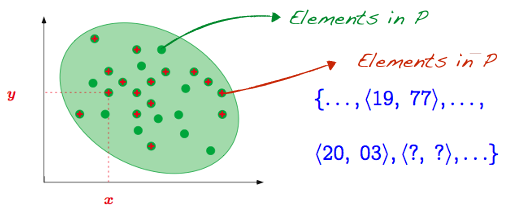
\includegraphics[scale=0.5]{img/approx.png}
\end{figure}
Per rispondere alla domanda $\langle x, y \rangle \in P$ utilizziamo un'astrazione $\bar{P}$,
tale che $P \supseteq \bar{P}$.
\begin{itemize}
  \item Se $\langle x, y \rangle \in \bar{P}$, quindi $d \subseteq d^\sharp$, allora $\langle x, y \rangle \in P$.
  \item Se $\langle x, y \rangle \notin \bar{P}$, quindi $d \supseteq d^\sharp$, allora non lo sappiamo.
\end{itemize}
In sintesi prendiamo un insieme più piccolo che comprende una sottoparte del nostro insieme di partenza e
analizziamo tale insieme più piccolo. Se troviamo una risposta positiva allora abbiamo risposto alla domanda,
altrimenti non lo sappiamo.
\subsection{Approssimazione dall'alto}
\begin{figure}[H]
  \centering
  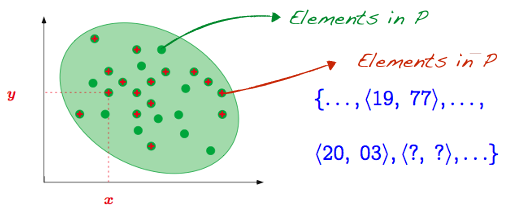
\includegraphics[scale=0.5]{img/approx.png}
\end{figure}
Per rispondere alla domanda $\langle x, y \rangle \in P$ utilizziamo un'astrazione $\bar{P}$,
tale che $P \subseteq \bar{P}$.
\begin{itemize}
  \item Se $\langle x, y \rangle \in \bar{P}$, quindi $d \supseteq d^\sharp$, allora non sappiamo rispondere.
  \item Se $\langle x, y \rangle \notin \bar{P}$, quindi $d \subseteq d^\sharp$, allora no.
\end{itemize}
In sintesi prendiamo un insieme più grande che comprende il nostro insieme di partenza e
analizziamo tale insieme più grande. Più grande non è sinonimo di più complesso, ma spesso 
ricondurci a proprietà più generali potrebbe aiutarci nell'analisi, la rappresentazione estensionale 
potrebbe quindi risultare più semplice. Tale approccio ci permette 
di rispondere alla domanda solo che la proprietà non è soddisfatta per il nuovo insieme più grande, 
ovvero $P^\sharp$.

In sostanza:
\begin{tcolorbox}[title=Proprietà concrete]
Le proprietà concrete sono un insieme di oggetti potenzialmente complessi, infiniti e non rappresentabili
da un calcolatore.
\end{tcolorbox}

\begin{tcolorbox}[title=Proprietà astratte]
  Le proprietà astratte sono un insieme più ampio di oggetti. A volte, l'ampiezza maggiore
  implica una maggiore estensibilità per la rappresentazione. Tuttavia, strutture più ampie
  ben scelte possono
  avere codifiche più semplici che possono essere sfruttate per la memorizzazione e il calcolo.
\end{tcolorbox}
\subsection{Minima astrazione}
Assumendo che le proprietà astratte $P \in \wp(\Sigma)$ devono essere apporssimate 
dall'alto della proprietà astratta $\bar{P} \in A \subset \wp(\Sigma)$, tale che:
\[
  P \subseteq \bar{P}
\]
Sappiamo che la più piccola proprietà $\bar{P}$ è la più precisa delle approssimazioni che possiamo avere.
Ovviamente, la minima proprietà astratta potrebbe non non esistere per tutte le astrazioni $A$.
Se questa minima approssimazione esiste è preferibile che sia il più precisa possibile, se non esiste,
può essere utilizzata una
migliore alternativa che fornisce un'approssimazione più precisa.
\subsection{Miglior astrazione}
Una buona scelta per l'astrazione è quella che fornisce la
miglior approssimazione per ogni proprietà concreta
\[
  P \subseteq \bar{P}
\]
\[
  \forall \bar{P}' \in A . (P \subseteq \bar{P}') \implies (\bar{P} \subseteq \bar{P}')
\]
Segue che la miglior approssimazione è la \textit{greatest lower bound} di tutte le approssimazioni
delle proprietà.
\[
\bar{P} = \bigcap \{\bar{P}' \in A \mid P \subseteq \bar{P}'\} \in A
\]
Tra tutti gli elementi più piccoli di quelli in $X$, è il più grande.
\[
  x = \texttt{glb}X \subseteq P \iff \forall l \in P . (\forall y \in X. l \leq y) \implies x \geq l
\]
\subsection{Esempio: \texttt{Sign}}
\subsubsection{Semantica concreta}
Abbiamo a disposizione programmi che manipolano numeri interi: \(f: \mathbb{Z} \to \mathbb{Z}\). Una delle 
proprietà osservate è quella di \textit{sign}, ovvero che il risultato tra due numeri dipenderà dal segno
dei due numeri. Dobbiamo indicare cosa inseriremo in $D^\sharp$ ovvero \texttt{Sign}.
\begin{itemize}
  \item $+ = \{n \mid n > 0\} \in \wp(\mathbb{Z})$
  \item $- = \{n \mid n < 0\} \in \wp(\mathbb{Z})$
  \item $0 = \{0\} \in \wp(\mathbb{Z})$
\end{itemize}
Quindi:
\[
  \{+, 0, -\} \subseteq \wp(\mathbb{Z})
\] 

\subsubsection{Semantica astratta}
Il dominio astratto, noto come \texttt{Sign}, viene utilizzato per approssimare
l'insieme di interi manipolati dai programmi. La funzione $f^\sharp$ manipola quindi i segni. 
\[
  D^\sharp = \{+, -, 0, \mathbb{Z}, \varnothing\} = \texttt{Sign}
\]
In \texttt{Sign},
gli interi possono essere rappresentati come:

\begin{itemize}
  \item $x \subseteq \mathbb{Z} \rightarrow x^\sharp \in D^\sharp$ è il più piccolo 
  insieme in $D^\sharp$ che contiene $x$.
  \item \(\{-,5,4 \} \rightarrow \mathbb{Z}\)
  \item \(\{ 3 \} \rightarrow + \equiv \mathbb{Z}\)
  \item \(\{ 7 \}  \rightarrow + \equiv \mathbb{Z}^{+}\)
  \item \(\{-5 \} \rightarrow - \equiv \mathbb{Z}^{-}\)
  \item \( \{ -5, -6 \} \rightarrow - \equiv \mathbb{Z}^{-}\)
\end{itemize}
\begin{minipage}[t]{0.4\textwidth}
  \begin{figure}[H]
  \centering
  \renewcommand{\arraystretch}{2}
  \begin{tabular}{|m{2em}|m{2em}|m{2em}|m{2em}|m{2em}|m{2em}|}
      \hline
       & $\mathbb{Z}$ & $\mathbb{Z}^+$ & $\mathbb{Z}^0$ & $\mathbb{Z}^-$ & $\varnothing$ \\
      \hline
      $\mathbb{Z}$ & $\mathbb{Z}$ & $\mathbb{Z}$ & $\mathbb{Z}$ & $\mathbb{Z}$ & $\mathbb{Z}$ \\
      \hline
      $\mathbb{Z}^+$ & $\mathbb{Z}$ & $\mathbb{Z}^+$ & $\mathbb{Z}^+$ & \textcolor{red}{$\mathbb{Z}$} & $\mathbb{Z}^+$ \\
      \hline
      $\mathbb{Z}^0$ & $\mathbb{Z}$ & $\mathbb{Z}^+$ & $\mathbb{Z}^0$ & $\mathbb{Z}^-$ & $\mathbb{Z}^0$ \\
      \hline
      $\mathbb{Z}^-$ & \textcolor{red}{$\mathbb{Z}$}  & $\mathbb{Z}$ & $\mathbb{Z}^-$ & $\mathbb{Z}^-$ & $\mathbb{Z}^-$ \\
      \hline
      $\varnothing$ & $\mathbb{Z}$ & $\mathbb{Z}^+$ & $\mathbb{Z}^0$ & $\mathbb{Z}^-$ & $\varnothing$ \\
      \hline
    \end{tabular}
    \caption{Operazioni di \texttt{Sign} relative alla somma.}
  \end{figure}
\end{minipage}
\hfill
\begin{minipage}[t]{0.5\textwidth}
  \begin{figure}[H]
    \centering
    \renewcommand{\arraystretch}{2}
    \begin{tabular}{|m{2em}|m{2em}|m{2em}|m{2em}|m{2em}|m{2em}|}
        \hline
        & $\mathbb{Z}$ & $\mathbb{Z}^+$ & $\mathbb{Z}^0$ & $\mathbb{Z}^-$ & $\varnothing$ \\
        \hline
        $\mathbb{Z}$ & $\mathbb{Z}$ & $\mathbb{Z}$ & $\mathbb{Z}$ & $\mathbb{Z}$ & $\mathbb{Z}$ \\
        \hline
        $\mathbb{Z}^+$ & $\mathbb{Z}$ & $\mathbb{Z}^+$ & $\mathbb{Z}^0$ & $\mathbb{Z}^-$ & $\mathbb{Z}^+$ \\
        \hline
        $\mathbb{Z}^0$ & $\mathbb{Z}$ & $\mathbb{Z}^0$ & $\mathbb{Z}^0$ & $\mathbb{Z}^0$ & $\mathbb{Z}^0$ \\
        \hline
        $\mathbb{Z}^-$ & $\mathbb{Z}$ & $\mathbb{Z}^-$ & $\mathbb{Z}^0$ & $\mathbb{Z}^+$ & $\mathbb{Z}^-$ \\
        \hline
        $\varnothing$ & $\mathbb{Z}$ & $\mathbb{Z}^+$ & $\mathbb{Z}^0$ & $\mathbb{Z}^-$ & $\varnothing$ \\
        \hline
    \end{tabular}
    \caption{Operazioni di \texttt{Sign} relative alla moltiplicazione.}
  \end{figure}
\end{minipage}

Per quanto riguarda la somma perdiamo informazioni solamente nel caso in cui si abbia un'operazione tra 
un numero positivo e uno negativo, poiché perdiamo le informazioni relative ai valori. Per quanto riguarda la moltiplicazione, invece, non perdiamo informazioni 
guardando la proprietà \texttt{Sign}, poiché è precisa sulla moltiplicazione.
\section{Astrazione delle computazioni}
Si tratta di approssimare la semantica sul dominio delle osservazioni.
Una volta fissate queste osservazioni, osserviamo come la semantica opera su di esse.

Abbiamo già visto il significato di computazione, che ripetiamo.
\begin{tcolorbox}[title = {Computazione}]
  Una computazione è una traccia nel tempo dello stato del programma durante l'esecuzione. Quindi lo stato 
  delle memorie nei vari punti del programma.
  A partire da uno stato iniziale noi abbiamo le possibili traiettorie di esecuzione del programma, 
  talvolta infinite 
  poiché potenzialmente divergenti.
\end{tcolorbox}
In realtà le possibili traiettorie non sono continue, ma sono discrete, poiché fissiamo degli step di tempo 
che tipicamente corrispondono alle singole istruzioni del programma e ogni traccia è spezzata in questa sequenza 
di evoluzione.

\subsection{Computazione di insiemi}
Quello che avviene ricerca della \textbf{decidibilità} è quello di osservare le proprietà di interesse.
Per osservare le proprietà di interesse, necessitiamo dell'osservazione di insiemi. L'insieme infatti 
rappresenta una proprietà che descrive un invariante di tutti gli elementi in esso contenuti.

Trasformando l'insieme di tracce in un'unica computazione che avviene tra insiemi. I punti rimangono comunque 
concreti, quindi dal punto di vista di ciò che possiamo calcolare, ovvero degli stati raggiungibili ad 
ogni passo di computazione, non cambia nulla, perché non perdiamo informazioni sugli stati raggiunti. 

Questo calcolo però non vogliamo eseguirlo con il calcolo diretto, perché l'infinità delle traiettorie non 
viene assolutamente alterata, quindi stiamo potenzialmente gestendo insiemi potenzialmente infiniti.
\begin{figure}[H]
  \centering
  \begin{tikzpicture}[->,>=stealth,thick,node distance=3cm]
    \node[ellipse,draw,fill=blue!20,minimum width=1cm, minimum height=5cm] (A) {};
    \node[ellipse,draw,fill=red!20,minimum width=1cm, minimum height=5cm] (B) at (2,0) {};
    \node[ellipse,draw,fill=green!20,minimum width=1cm, minimum height=5cm] (C) at (4,0) {};
    \node[ellipse,draw,fill=orange!20,minimum width=1cm, minimum height=5cm] (D) at (6,0) {};
    \node[ellipse,draw,fill=yellow!20,minimum width=1cm, minimum height=5cm] (E) at (8,0) {};
    \node[ellipse,draw,fill=purple!20,minimum width=1cm, minimum height=5cm] (F) at (10,0) {};
    \node[ellipse,draw,fill=cyan!20,minimum width=1cm, minimum height=5cm] (G) at (12,0) {};
    \node (A1) at (13.4,0) {\dots};
  
    \pgfmathsetmacro{\increment}{0}
  
    \foreach \i in {1,...,10}
    {
        \fill (A.center) + (\increment,2*rand) circle (2pt);
        \fill (B.center) + (\increment,2*rand) circle (2pt);
        \fill (C.center) + (\increment,2*rand) circle (2pt);
        \fill (D.center) + (\increment,2*rand) circle (2pt);
        \fill (E.center) + (\increment,2*rand) circle (2pt);
        \fill (F.center) + (\increment,2*rand) circle (2pt);
        \fill (G.center) + (\increment,2*rand) circle (2pt);
    }
  
    \path[every node/.style={font=\sffamily\small}]
      (A) edge[] node[above] {} (B)
      (B) edge[] node[above] {} (C)
      (C) edge[] node[above] {} (D)
      (D) edge[] node[above] {} (E)
      (E) edge[] node[above] {} (F)
      (F) edge[] node[above] {} (G)
      (G) edge[] node[above] {} (13,0);
  
    % asse x
    \draw[->] (0,-3) -- (13,-3) node[right] {$t$};
    % asse y
    \draw[->] (0,-3) -- (0,4) node[above] {$x(t)$};
  \end{tikzpicture}
  \caption{Traccia di una computazione di insiemi.}
\end{figure}

Il calcolo avviene quindi per punto fisso, partiamo quindi da un insieme di stati iniziali e andiamo via a via 
a collezionare tutti gli stati che raggiungiamo durante l'esecuzione, chiamato \textbf{reachability semantics} o
\textbf{collecting semantics}.

\subsection{Collecting semantics}
Dal punto di vista della raggiungibilità degli stati, l'informazione è precisa, infatti l'insieme di stati
raggiunti sono gli stessi che avremmo raggiunto con la semantica concreta. Di fatto, però, abbiamo una perdita 
di informazione dal punto di vista dell'insieme delle tracce che stiamo rappresentando.

\begin{figure}[H]
  \centering
  \begin{tikzpicture}[-,>=stealth,thick,node distance=3cm]

    \draw[] (1,3) -- (3,3) node[right] {};
    \draw[] (1,2) -- (5,2) node[right] {};
    \draw[] (1,1) -- (7,1) node[right] {};
    \draw[] (1,0) -- (6,0) node[right] {};

    \fill[blue!80,draw=black] (1,3) circle (2pt);
    \fill[red!80,draw=black] (1,2) circle (2pt);
    \fill[green!90,draw=black] (1,1) circle (2pt);
    \fill[cyan!80,draw=black] (1,0) circle (2pt);
  
    \fill[blue!60,draw=black] (2,3) circle (2pt);
    \fill[red!70,draw=black] (2,2) circle (2pt);
    \fill[green!80,draw=black] (2,1) circle (2pt);
    \fill[cyan!70,draw=black] (2,0) circle (2pt);
  
    \fill[blue!40,draw=black] (3,3) circle (2pt);
    \fill[red!60,draw=black] (3,2) circle (2pt);
    \fill[green!70,draw=black] (3,1) circle (2pt);
    \fill[cyan!60,draw=black] (3,0) circle (2pt);
  
    \fill[red!50,draw=black] (4,2) circle (2pt);
    \fill[green!60,draw=black] (4,1) circle (2pt);
    \fill[cyan!50,draw=black] (4,0) circle (2pt);
  
    \fill[red!40,draw=black] (5,2) circle (2pt);
    \fill[green!50,draw=black] (5,1) circle (2pt);
    \fill[cyan!40,draw=black] (5,0) circle (2pt);
  
    \fill[green!40,draw=black] (6,1) circle (2pt);
    \fill[cyan!30,draw=black] (6,0) circle (2pt);
  
    \fill[green!30,draw=black] (7,1) circle (2pt);

    \draw[decorate, decoration= {calligraphic brace}] (0,0) -- (0,3);
    \draw[decorate, decoration= {calligraphic brace}] (8,3) -- (8,0)
    node[midway,right,xshift=0.5cm] {Tracce semantiche};

    \node[ellipse,draw, fill=white, minimum width=0.7, minimum height=3cm] (A) at (1,-3) {};
    \node[ellipse,draw, fill=white, minimum width=0.7, minimum height=3cm] (B) at (2,-3) {};
    \node[ellipse,draw, fill=white, minimum width=0.7, minimum height=3cm] (C) at (3,-3) {};
    \node[ellipse,draw, fill=white, minimum width=0.7, minimum height=3cm] (D) at (4,-3) {};
    \node[ellipse,draw, fill=white, minimum width=0.7, minimum height=3cm] (E) at (5,-3) {};
    \node[ellipse,draw, fill=white, minimum width=0.7, minimum height=3cm] (F) at (6,-3) {};
    \node[ellipse,draw, fill=white, minimum width=0.7, minimum height=3cm] (G) at (7,-3) {};

    \fill[blue!80,draw=black] (1,-2) circle (2pt);
    \fill[red!80,draw=black] (1,-2.5) circle (2pt);
    \fill[green!90,draw=black] (1,-3) circle (2pt);
    \fill[cyan!80,draw=black] (1,-3.5) circle (2pt);
  
    \fill[blue!60,draw=black] (2,-2) circle (2pt);
    \fill[red!70,draw=black] (2,-2.5) circle (2pt);
    \fill[green!80,draw=black] (2,-3) circle (2pt);
    \fill[cyan!70,draw=black] (2,-3.5) circle (2pt);
  
    \fill[blue!40,draw=black] (3,-2) circle (2pt);
    \fill[red!60,draw=black] (3,-2.5) circle (2pt);
    \fill[green!70,draw=black] (3,-3) circle (2pt);
    \fill[cyan!60,draw=black] (3,-3.5) circle (2pt);
  
    \fill[red!50,draw=black] (4,-2.7) circle (2pt);
    \fill[green!60,draw=black] (4,-3.0) circle (2pt);
    \fill[cyan!50,draw=black] (4,-3.3) circle (2pt);
  
    \fill[red!40,draw=black] (5,-2.7) circle (2pt);
    \fill[green!50,draw=black] (5,-3.0) circle (2pt);
    \fill[cyan!40,draw=black] (5,-3.3) circle (2pt);
  
    \fill[green!40,draw=black] (6,-2.8) circle (2pt);
    \fill[cyan!30,draw=black] (6,-3.2) circle (2pt);
  
    \fill[green!30,draw=black] (7,-3) circle (2pt);  

    \draw[] (A) -- (B);
    \draw[] (B) -- (C);
    \draw[] (C) -- (D);
    \draw[] (D) -- (E);
    \draw[] (E) -- (F);
    \draw[] (F) -- (G);
  \end{tikzpicture}
\end{figure}

La semantica delle tracce mi colleziona l'insieme di tutte le tracce di computazione e 
la semantica delle collezioni invece considera per ogni passo di computazione l'insieme 
la proprietà raggiunta degli stati raggiunti.
Abbiamo perso informazione rispetto alle tracce che rappresentiamo, in questo passaggio 
perdiamo la traccia che nello stato successivo raggiunge un determinato stato, poiché la traccia 
diventa unica.

\begin{figure}[H]
  \centering
  \begin{tikzpicture}[-,>=stealth,thick,node distance=3cm]

    \draw[] (1,3) -- (3,3) node[right] {};
    \draw[] (1,2) -- (5,2) node[right] {};
    \draw[] (1,1) -- (7,1) node[right] {};
    \draw[] (1,0) -- (6,0) node[right] {};

    \draw[draw=red] (1,0) -- (2,2) node[right] {};
    \draw[draw=red] (2,2) -- (3,3) node[right] {};
    \draw[draw=red] (3, 3) -- (4,1) node[right] {};
    \draw[draw=red] (4,1) -- (5,2) node[right] {};
    \draw[draw=red] (5,2) -- (6,0) node[right] {};
    \draw[draw=red] (6,0) -- (7,1) node[right] {};

    \fill[blue!80,draw=black] (1,3) circle (2pt);
    \fill[red!80,draw=black] (1,2) circle (2pt);
    \fill[green!90,draw=black] (1,1) circle (2pt);
    \fill[cyan!80,draw=black] (1,0) circle (2pt);
  
    \fill[blue!60,draw=black] (2,3) circle (2pt);
    \fill[red!70,draw=black] (2,2) circle (2pt);
    \fill[green!80,draw=black] (2,1) circle (2pt);
    \fill[cyan!70,draw=black] (2,0) circle (2pt);
  
    \fill[blue!40,draw=black] (3,3) circle (2pt);
    \fill[red!60,draw=black] (3,2) circle (2pt);
    \fill[green!70,draw=black] (3,1) circle (2pt);
    \fill[cyan!60,draw=black] (3,0) circle (2pt);
  
    \fill[red!50,draw=black] (4,2) circle (2pt);
    \fill[green!60,draw=black] (4,1) circle (2pt);
    \fill[cyan!50,draw=black] (4,0) circle (2pt);
  
    \fill[red!40,draw=black] (5,2) circle (2pt);
    \fill[green!50,draw=black] (5,1) circle (2pt);
    \fill[cyan!40,draw=black] (5,0) circle (2pt);
  
    \fill[green!40,draw=black] (6,1) circle (2pt);
    \fill[cyan!30,draw=black] (6,0) circle (2pt);
  
    \fill[green!30,draw=black] (7,1) circle (2pt);

    \draw[decorate, decoration= {calligraphic brace}] (0,0) -- (0,3);
    \draw[decorate, decoration= {calligraphic brace}] (8,3) -- (8,0)
    node[midway,right,xshift=0.5cm] {Tracce semantiche};

  \end{tikzpicture}
\end{figure}
Abbiamo buttato via l'informazione che riguardava l'esatta transizione tra gli stati, aggiungendo tracce 
spurie.

La domanda che sporge spontanea è se ci stiamo muovendo nella direzione della 
decidibilità; di fatto no. Vediamo quindi un'altra rappresentazione che ci permette di comprendere 
la situazione.
\begin{figure}[H]
  \centering
  \begin{tikzpicture}[-,>=stealth,thick,node distance=3cm]

    \draw[dashed] (1,0) -- (1,5);
        \draw[dashed] (2,0) -- (2,5);
        \draw[dashed] (3,0) -- (3,5);
        \draw[dashed] (4,0) -- (4,5);
        \draw[dashed] (5,0) -- (5,5);
        \draw[dashed] (6,0) -- (6,5);
        \draw[dashed] (7,0) -- (7,5);
        \draw[dashed] (8,0) -- (8,5);
        \draw[dashed] (9,0) -- (9,5);
        \draw[dashed] (10,0) -- (10,5);

    \fill[blue!80,draw=black] (1,5) circle (3pt);
    \fill[blue!70,draw=black] (1,4) circle (3pt);
    \fill[blue!60,draw=black] (1,3) circle (3pt);
    \fill[blue!50,draw=black] (1,2) circle (3pt);
    \fill[blue!40,draw=black] (1,1) circle (3pt);
    \fill[blue!30,draw=black] (1,0) circle (3pt);
  
    \fill[green!80,draw=black] (2,5) circle (3pt);
    \fill[green!70,draw=black] (2,4) circle (3pt);
    \fill[green!60,draw=black] (2,3) circle (3pt);
    \fill[green!50,draw=black] (2,2) circle (3pt);
    \fill[green!40,draw=black] (2,1) circle (3pt);
    \fill[green!30,draw=black] (2,0) circle (3pt);
  
    \fill[purple!80,draw=black] (3,5) circle (3pt);
    \fill[purple!70,draw=black] (3,4) circle (3pt);
    \fill[purple!60,draw=black] (3,3) circle (3pt);
    \fill[purple!50,draw=black] (3,2) circle (3pt);
    \fill[purple!40,draw=black] (3,1) circle (3pt);
    \fill[purple!30,draw=black] (3,0) circle (3pt);

    \fill[red!80,draw=black] (4,5) circle (3pt);
    \fill[brown!70,draw=black] (4,4) circle (3pt);
    \fill[brown!60,draw=black] (4,3) circle (3pt);
    \fill[brown!50,draw=black] (4,2) circle (3pt);
    \fill[brown!40,draw=black] (4,1) circle (3pt);
    \fill[pink,draw=black] (4,0) circle (3pt);

    \fill[gray!70,draw=black] (5,4) circle (3pt);
    \fill[gray!60,draw=black] (5,3) circle (3pt);
    \fill[gray!50,draw=black] (5,2) circle (3pt);
    \fill[gray!40,draw=black] (5,1) circle (3pt);
    \fill[gray!30,draw=black] (5,0) circle (3pt);

    \fill[red!80,draw=black] (6,4) circle (3pt);
    \fill[purple!60,draw=black] (6,3) circle (3pt);
    \fill[purple!50,draw=black] (6,2) circle (3pt);
    \fill[purple!40,draw=black] (6,1) circle (3pt);
    \fill[purple!30,draw=black] (6,0) circle (3pt);

    \fill[brown!60,draw=black] (7,3) circle (3pt);
    \fill[brown!50,draw=black] (7,2) circle (3pt);
    \fill[brown!40,draw=black] (7,1) circle (3pt);
    \fill[yellow!80,draw=black] (7,0) circle (3pt);

    \fill[red!80,draw=black] (8,3) circle (3pt);
    \fill[green!50,draw=black] (8,2) circle (3pt);
    \fill[green!40,draw=black] (8,1) circle (3pt);

    \fill[purple!50,draw=black] (9,2) circle (3pt);
    \fill[red!80,draw=black] (9,1) circle (3pt);

    \fill[yellow!80,draw=black] (10,2) circle (3pt);

    \draw[decorate, decoration={calligraphic brace, amplitude=6pt, mirror, raise=5pt, aspect=0.5}]
    (11,-0.5) -- (11,5) node[midway,right,xshift=0.5cm] {Tracce semantiche};

    % Labels for the dashed lines
    \node at (1,-0.5) {1};
    \node at (2,-0.5) {2};
    \node at (3,-0.5) {3};
    \node at (4,-0.5) {4};
    \node at (5,-0.5) {5};
    \node at (6,-0.5) {6};
    \node at (7,-0.5) {7};
    \node at (8,-0.5) {8};
    \node at (9,-0.5) {9};
    \node at (10,-0.5) {10};
  \end{tikzpicture}
\end{figure}
Ad ogni passo di computazione eseguiamo un istruzione in un \textbf{punto di programma}, possiamo 
quindi guardare il punto di programma che stiamo osservando.

\begin{figure}[H]
  \centering
  \begin{tikzpicture}[-,>=stealth,thick,node distance=3cm]

    \draw[dashed] (1,0) -- (1,5);
        \draw[dashed] (2,0) -- (2,5);
        \draw[dashed] (3,0) -- (3,5);
        \draw[dashed] (4,0) -- (4,5);
        \draw[dashed] (5,0) -- (5,5);
        \draw[dashed] (6,0) -- (6,5);
        \draw[dashed] (7,0) -- (7,5);
        \draw[dashed] (8,0) -- (8,5);
        \draw[dashed] (9,0) -- (9,5);
        \draw[dashed] (10,0) -- (10,5);

    \fill[blue!80,draw=black] (1,5) circle (3pt);
    \fill[blue!70,draw=black] (1,4) circle (3pt);
    \fill[blue!60,draw=black] (1,3) circle (3pt);
    \fill[blue!50,draw=black] (1,2) circle (3pt);
    \fill[blue!40,draw=black] (1,1) circle (3pt);
    \fill[blue!30,draw=black] (1,0) circle (3pt);
  
    \fill[green!80,draw=black] (2,5) circle (3pt);
    \fill[green!70,draw=black] (2,4) circle (3pt);
    \fill[green!60,draw=black] (2,3) circle (3pt);
    \fill[green!50,draw=black] (2,2) circle (3pt);
    \fill[green!40,draw=black] (2,1) circle (3pt);
    \fill[green!30,draw=black] (2,0) circle (3pt);
  
    \fill[purple!80,draw=black] (3,5) circle (3pt);
    \fill[purple!70,draw=black] (3,4) circle (3pt);
    \fill[purple!60,draw=black] (3,3) circle (3pt);
    \fill[purple!50,draw=black] (3,2) circle (3pt);
    \fill[purple!40,draw=black] (3,1) circle (3pt);
    \fill[purple!30,draw=black] (3,0) circle (3pt);

    \fill[red!80,draw=black] (4,5) circle (3pt);
    \node[red!80,right] at (4,5) {5};
    \fill[brown!70,draw=black] (4,4) circle (3pt);
    \fill[brown!60,draw=black] (4,3) circle (3pt);
    \fill[brown!50,draw=black] (4,2) circle (3pt);
    \fill[brown!40,draw=black] (4,1) circle (3pt);
    \fill[pink,draw=black] (4,0) circle (3pt);

    \fill[gray!70,draw=black] (5,4) circle (3pt);
    \fill[gray!60,draw=black] (5,3) circle (3pt);
    \fill[gray!50,draw=black] (5,2) circle (3pt);
    \fill[gray!40,draw=black] (5,1) circle (3pt);
    \fill[gray!30,draw=black] (5,0) circle (3pt);

    \fill[red!80,draw=black] (6,4) circle (3pt);
    \node[red!80,right] at (6, 4) {5};
    \fill[purple!60,draw=black] (6,3) circle (3pt);
    \fill[purple!50,draw=black] (6,2) circle (3pt);
    \fill[purple!40,draw=black] (6,1) circle (3pt);
    \fill[purple!30,draw=black] (6,0) circle (3pt);

    \fill[brown!60,draw=black] (7,3) circle (3pt);
    \fill[brown!50,draw=black] (7,2) circle (3pt);
    \fill[brown!40,draw=black] (7,1) circle (3pt);
    \fill[yellow!80,draw=black] (7,0) circle (3pt);

    \fill[red!80,draw=black] (8,3) circle (3pt);
    \node[red!80,right] at (8,3) {5};
    \fill[green!50,draw=black] (8,2) circle (3pt);
    \fill[green!40,draw=black] (8,1) circle (3pt);

    \fill[purple!50,draw=black] (9,2) circle (3pt);
    \fill[red!80,draw=black] (9,1) circle (3pt);
    \node[red!80,right] at (9,1) {5};

    \fill[yellow!80,draw=black] (10,2) circle (3pt);

    \draw[decorate, decoration={calligraphic brace, amplitude=6pt, mirror, raise=5pt, aspect=0.5}]
    (11,-0.5) -- (11,5) node[midway,right,xshift=0.5cm] {Tracce semantiche};

    % Labels for the dashed lines
    \node[blue!80] at (1,-0.5) {1};
    \node[green!80] at (2,-0.5) {2};
    \node[purple!80] at (3,-0.5) {3};
    \node[brown!80] at (4,-0.5) {4};
    \node[green!80] at (5,-0.5) {2};
    \node[purple!80] at (6,-0.5) {3};
    \node[brown!80] at (7,-0.5) {4};
    \node[green!80] at (8,-0.5) {2};
    \node[purple!80] at (9,-0.5) {3};
    \node[brown!50] at (10,-0.5) {4};
  \end{tikzpicture}
\end{figure}
Quello che osserviamo è che $5$ è uno stato terminale, e che i punti $2$ e $3$ sono 
il corpo del ciclo, andando avanti nel tempo 
torniamo a visitate dei  punti di programma.

Spostiamo la discretizzazione del punto di vista della traccia dal tempo ai punti di programma.

\begin{figure}[H]
  \centering
  \begin{tikzpicture}[-,>=stealth,thick,node distance=3cm]

    \draw[dashed] (1,0) -- (1,5);
        \draw[dashed] (2,0) -- (2,5);
        \draw[dashed] (3,0) -- (3,5);
        \draw[dashed] (4,0) -- (4,5);
        \draw[dashed] (5,0) -- (5,5);
        \draw[dashed] (6,0) -- (6,5);
        \draw[dashed] (7,0) -- (7,5);
        \draw[dashed] (8,0) -- (8,5);
        \draw[dashed] (9,0) -- (9,5);
        \draw[dashed] (10,0) -- (10,5);

    \fill[blue!80,draw=black] (1,5) circle (3pt);
    \fill[blue!70,draw=black] (1,4) circle (3pt);
    \fill[blue!60,draw=black] (1,3) circle (3pt);
    \fill[blue!50,draw=black] (1,2) circle (3pt);
    \fill[blue!40,draw=black] (1,1) circle (3pt);
    \fill[blue!30,draw=black] (1,0) circle (3pt);
  
    \fill[green!80,draw=black] (2,5) circle (3pt);
    \fill[green!70,draw=black] (2,4) circle (3pt);
    \fill[green!60,draw=black] (2,3) circle (3pt);
    \fill[green!50,draw=black] (2,2) circle (3pt);
    \fill[green!40,draw=black] (2,1) circle (3pt);
    \fill[green!30,draw=black] (2,0) circle (3pt);
  
    \fill[purple!80,draw=black] (3,5) circle (3pt);
    \fill[purple!70,draw=black] (3,4) circle (3pt);
    \fill[purple!60,draw=black] (3,3) circle (3pt);
    \fill[purple!50,draw=black] (3,2) circle (3pt);
    \fill[purple!40,draw=black] (3,1) circle (3pt);
    \fill[purple!30,draw=black] (3,0) circle (3pt);

    \fill[red!80,draw=black] (4,5) circle (3pt);
    \node[red!80,right] at (4,5) {5};
    \fill[brown!70,draw=black] (4,4) circle (3pt);
    \fill[brown!60,draw=black] (4,3) circle (3pt);
    \fill[brown!50,draw=black] (4,2) circle (3pt);
    \fill[brown!40,draw=black] (4,1) circle (3pt);
    \fill[pink,draw=black] (4,0) circle (3pt);

    \fill[gray!70,draw=black] (5,4) circle (3pt);
    \fill[gray!60,draw=black] (5,3) circle (3pt);
    \fill[gray!50,draw=black] (5,2) circle (3pt);
    \fill[gray!40,draw=black] (5,1) circle (3pt);
    \fill[gray!30,draw=black] (5,0) circle (3pt);

    \fill[red!80,draw=black] (6,4) circle (3pt);
    \node[red!80,right] at (6, 4) {5};
    \fill[purple!60,draw=black] (6,3) circle (3pt);
    \fill[purple!50,draw=black] (6,2) circle (3pt);
    \fill[purple!40,draw=black] (6,1) circle (3pt);
    \fill[purple!30,draw=black] (6,0) circle (3pt);

    \fill[brown!60,draw=black] (7,3) circle (3pt);
    \fill[brown!50,draw=black] (7,2) circle (3pt);
    \fill[brown!40,draw=black] (7,1) circle (3pt);
    \fill[yellow!80,draw=black] (7,0) circle (3pt);

    \fill[red!80,draw=black] (8,3) circle (3pt);
    \node[red!80,right] at (8,3) {5};
    \fill[green!50,draw=black] (8,2) circle (3pt);
    \fill[green!40,draw=black] (8,1) circle (3pt);

    \fill[purple!50,draw=black] (9,2) circle (3pt);
    \fill[red!80,draw=black] (9,1) circle (3pt);
    \node[red!80,right] at (9,1) {5};

    \fill[yellow!80,draw=black] (10,2) circle (3pt);

    \draw[decorate, decoration={calligraphic brace, amplitude=6pt, mirror, raise=5pt, aspect=0.5}]
    (11,-0.5) -- (11,5) node[midway,right,xshift=0.5cm] {Tracce semantiche};

    \draw[rounded corners=15pt]
        (0.5,-2) rectangle ++(1,-4);
        \fill[blue!80,draw=black] (1.2,-4.8) circle (3pt);
        \fill[blue!70,draw=black] (0.8, -5) circle (3pt);
        \fill[blue!60,draw=black] (1.2, -5.2) circle (3pt);
        \fill[blue!50,draw=black] (0.8,-5.4) circle (3pt);
        \fill[blue!40,draw=black] (1.2,-5.6) circle (3pt);
        \fill[blue!30,draw=black] (0.8,-5.8) circle (3pt);

    \draw[rounded corners=15pt]
        (1.5,-2) rectangle ++(1,-4);
        \fill[green!80,draw=black] (2.2,-4.8) circle (3pt);
        \fill[green!70,draw=black] (1.8, -5) circle (3pt);
        \fill[green!60,draw=black] (2.2, -5.2) circle (3pt);
        \fill[green!50,draw=black] (1.8,-5.4) circle (3pt);
        \fill[green!40,draw=black] (2.2,-5.6) circle (3pt);
        \fill[green!30,draw=black] (1.8,-5.8) circle (3pt);

        \fill[green!80,draw=black] (2.2,-4.5) circle (3pt);
        \fill[green!70,draw=black] (1.8, -4.4) circle (3pt);
        \fill[green!60,draw=black] (2.2, -4.2) circle (3pt);
        \fill[green!50,draw=black] (1.8,-4) circle (3pt);
        \fill[green!40,draw=black] (2.2,-3.8) circle (3pt);
        \fill[green!30,draw=black] (1.8,-3.6) circle (3pt);
        \fill[green!80,draw=black] (2.2,-3.4) circle (3pt);

    \draw[rounded corners=15pt]
        (2.5,-2) rectangle ++(1,-4);
        \fill[purple!80,draw=black] (3.2,-4.8) circle (3pt);
        \fill[purple!70,draw=black] (2.8, -5) circle (3pt);
        \fill[purple!60,draw=black] (3.2, -5.2) circle (3pt);
        \fill[purple!50,draw=black] (2.8,-5.4) circle (3pt);
        \fill[purple!40,draw=black] (3.2,-5.6) circle (3pt);
        \fill[purple!30,draw=black] (2.8,-5.8) circle (3pt);

        \fill[purple!80,draw=black] (3.2,-4.5) circle (3pt);
        \fill[purple!70,draw=black] (2.8, -4.4) circle (3pt);
        \fill[purple!60,draw=black] (3.2, -4.2) circle (3pt);
        \fill[purple!50,draw=black] (2.8,-4) circle (3pt);
        \fill[purple!40,draw=black] (3.2,-3.8) circle (3pt);
        \fill[purple!30,draw=black] (2.8,-3.6) circle (3pt);
        
    \draw[rounded corners=15pt]
        (3.5,-2) rectangle ++(1,-4);
        \fill[brown!70,draw=black] (3.8, -5) circle (3pt);
        \fill[brown!60,draw=black] (4.2, -5.2) circle (3pt);
        \fill[brown!50,draw=black] (3.8,-5.4) circle (3pt);
        \fill[brown!40,draw=black] (4.2,-5.6) circle (3pt);
        \fill[brown!30,draw=black] (3.8,-5.8) circle (3pt);

        \fill[brown!60,draw=black] (4.2, -4.5) circle (3pt);
        \fill[brown!50,draw=black] (3.8,-4.4) circle (3pt);
        \fill[brown!40,draw=black] (4.2,-4.2) circle (3pt);
        \fill[brown!30,draw=black] (3.8,-4) circle (3pt);

    \draw[rounded corners=15pt]
        (4.5,-2) rectangle ++(1,-4);
        \fill[red!80,draw=black] (4.8, -5.8) circle (3pt);
        \fill[red!80,draw=black] (5.2, -5.6) circle (3pt);
        \fill[red!80,draw=black] (4.8, -5.4) circle (3pt);
        \fill[red!80,draw=black] (5.2, -5.2) circle (3pt);
  \end{tikzpicture}
\end{figure}
Quello che viene fatto è quello di collezionare gli elementi nei punti di 
programma che sono stati eseguiti. Di fatto per ogni punto di programma, l'insieme 
degli stati è sempre incrementale rispetto al punto di programma.

Potenzialmente anche questa rappresentazione sarà non terminante, poiché stiamo 
guardando ancora il mondo concreto, quindi gli stati raggiungibili sono ancora potenzialmente
infiniti.
Soprattutto in presenza di un ciclo \texttt{while} che calcola valori differenti ad ogni iterazione.
\begin{algorithm}[H]
  $x \gets 0$

  \While{$x \geq  0$}{
    $x \gets x + 1$
  }
\end{algorithm}
L'insieme in questo caso continuerà ad espandersi all'infinito, poiché non c'è un limite e quindi
non è possibile trovare un punto fisso.
Il tentativo di raggiungere la terminazione è quello di trovare la stabilità di tali insiemi. 

In alcuni casi la decidibilità è raggiungibile, ma nella maggior pate dei casi non è possibile.
\begin{algorithm}[H]
  $x \gets 0$

  \While{$x \geq  0$}{
    $x \gets x$
  }
\end{algorithm}
In caso appena riportato l'insieme degli stati è sempre lo stesso, quindi è possibile trovare un punto fisso.
\subsection{Computazioni sulle proprietà}
Nella collecting semantics abbiamo quindi esecuzioni spurie, dovute al fatto che collezioniamo 
insiemi di stati, ma sono solo tra stati raggiungibili. Il fatto che manteniamo gli stati raggiungibili
fa si che non vi sia perdita di informazione, ma dall'altra parte abbiamo esecuzioni potenzialmente infinite.

Dobbiamo ulteriormente raffinare la collecting semantics, per poter raggiungere la terminazione. Per farlo 
abbiamo bisogno dell'approssimazione, non più calcolando sugli insiemi di stati raggiungibili, ma su proprietà 
degli stati raggiungibili. Spostiamo quindi l'attenzione sugli sulle proprietà aggiungendo ulteriore 
rumore.
\begin{figure}[H]
  \centering
  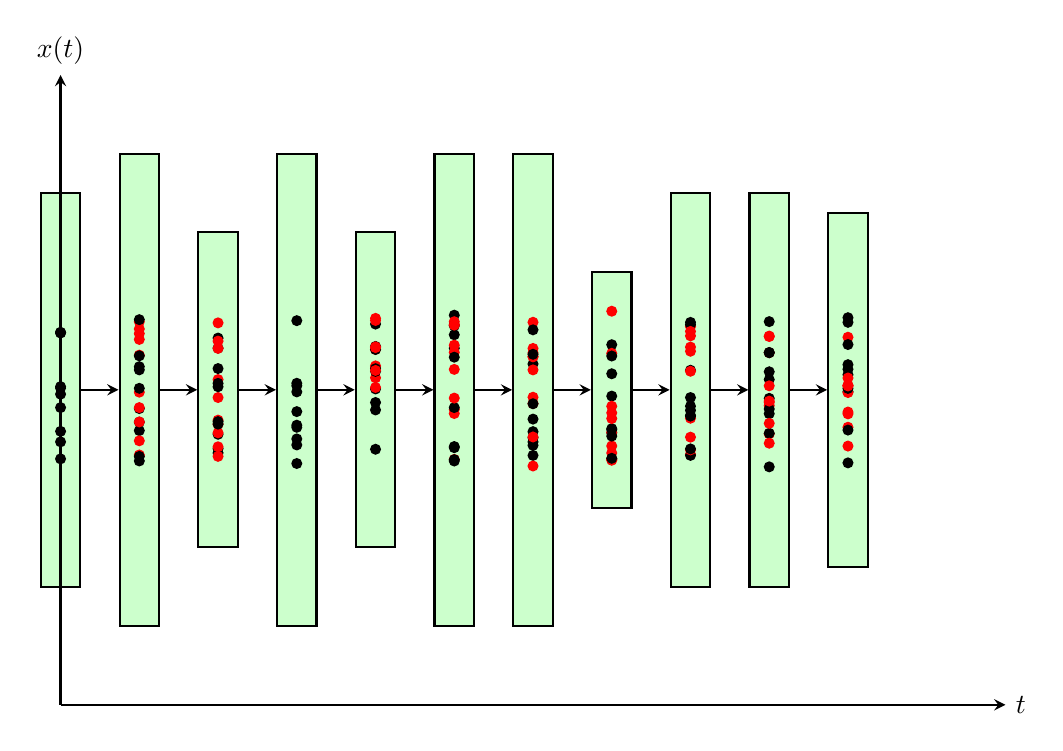
\begin{tikzpicture}[->,>=stealth,thick,node distance=3cm]
    \node[rectangle,draw,fill=green!20,minimum width=0.5cm, minimum height=5cm] (A) {};
    \node[rectangle,draw,fill=green!20,minimum width=0.5cm, minimum height=6cm] (B) at (1,0) {};
    \node[rectangle,draw,fill=green!20,minimum width=0.5cm, minimum height=4cm] (C) at (2,0) {};
    \node[rectangle,draw,fill=green!20,minimum width=0.5cm, minimum height=6cm] (D) at (3,0) {};
    \node[rectangle,draw,fill=green!20,minimum width=0.5cm, minimum height=4cm] (E) at (4,0) {};
    \node[rectangle,draw,fill=green!20,minimum width=0.5cm, minimum height=6cm] (F) at (5,0) {};
    \node[rectangle,draw,fill=green!20,minimum width=0.5cm, minimum height=6cm] (G) at (6,0) {};
    \node[rectangle,draw,fill=green!20,minimum width=0.5cm, minimum height=3cm] (H) at (7,0) {};
    \node[rectangle,draw,fill=green!20,minimum width=0.5cm, minimum height=5cm] (I) at (8,0) {};
    \node[rectangle,draw,fill=green!20,minimum width=0.5cm, minimum height=5cm] (J) at (9,0) {};
    \node[rectangle,draw,fill=green!20,minimum width=0.5cm, minimum height=4.5cm] (K) at (10,0) {};
  
    \pgfmathsetmacro{\increment}{0}
  
    \foreach \i in {1,...,10}
    {
        \fill (A.center) + (\increment,rand) circle (2pt);
        \fill (B.center) + (\increment,rand) circle (2pt);
        \fill (C.center) + (\increment,rand) circle (2pt);
        \fill (D.center) + (\increment,rand) circle (2pt);
        \fill (E.center) + (\increment,rand) circle (2pt);
        \fill (F.center) + (\increment,rand) circle (2pt);
        \fill (G.center) + (\increment,rand) circle (2pt);
        \fill (H.center) + (\increment,rand) circle (2pt);
        \fill (I.center) + (\increment,rand) circle (2pt);
        \fill (J.center) + (\increment,rand) circle (2pt);
        \fill (K.center) + (\increment,rand) circle (2pt);
        \fill[red] (B.center) + (\increment,rand) circle (2pt);
        \fill[red] (C.center) + (\increment, rand) circle (2pt);
        \fill[red] (E.center) + (\increment,rand) circle (2pt);
        \fill[red] (F.center) + (\increment,rand) circle (2pt);
        \fill[red] (G.center) + (\increment,rand) circle (2pt);
        \fill[red] (H.center) + (\increment,rand) circle (2pt);
        \fill[red] (I.center) + (\increment,rand) circle (2pt);
        \fill[red] (J.center) + (\increment,rand) circle (2pt);
        \fill[red] (K.center) + (\increment,rand) circle (2pt);
    }
  
    \path[every node/.style={font=\sffamily\small}]
      (A) edge node [left] {} (B)
      (B) edge node [left] {} (C)
      (C) edge node [left] {} (D)
      (D) edge node [left] {} (E)
      (E) edge node [left] {} (F)
      (F) edge node [left] {} (G)
      (G) edge node [left] {} (H)
      (H) edge node [left] {} (I)
      (I) edge node [left] {} (J)
      (J) edge node [left] {} (K);
  
    % asse x
    \draw[->] (0,-4) -- (12,-4) node[right] {$t$};
    % asse y
    \draw[->] (0,-4) -- (0,4) node[above] {$x(t)$};
  \end{tikzpicture}
  \caption{Traccia di una computazione sulle proprietà.}
  \label{fig:compupropr}
\end{figure}
Non abbiamo solamente computazioni spurie dovute al fatto che ci muoviamo tra insiemi, ma abbiamo 
computazioni spurie che partono da stati che non vengono mai raggiunti nel concreto (\textit{rappresentati 
dai pallini rossi nell'immagine} \ref{fig:compupropr}).

L'idea genera è quella di:
\begin{itemize}
  \item Passare da l'insieme di tracce distinte ad una taccia di insiemi rappresentate (\textit{che 
  aggiunge rumore, mediante tracce spurie}).
  \item A questo punto è possibile approssimare la computazione guardando proprietà, utilizzando quindi 
  la semantics collecting sulle proprietà, che possono agevolare la terminazione.
\end{itemize}